\documentclass[a4paper,11pt]{article}

% --- Encodage et Langue ---
\usepackage[utf8]{inputenc}
\usepackage[T1]{fontenc}
\usepackage[french]{babel}

% --- Mise en page et Typographie ---
\usepackage{geometry}
\geometry{margin=2.5cm, headheight=15pt}
\usepackage{microtype}
\usepackage{lmodern}

% --- En-têtes et pieds de page ---
\usepackage{fancyhdr}
\pagestyle{fancy}
\fancyhf{}
\renewcommand{\headrulewidth}{0pt}
\renewcommand{\footrulewidth}{0.4pt}
\fancyfoot[L]{\small\textcolor{primary}{\textit{Copyrights Jean-Christophe Le Lann -- Électronique Numérique}}}
\fancyfoot[R]{\small\textcolor{primary}{\thepage}}

% --- Mathématiques ---
\usepackage{amsmath, amssymb}
\usepackage{centernot}

% --- Images ---
\usepackage{graphicx}
\usepackage{float}

% --- Couleurs et Boîtes ---
\usepackage{xcolor}
\definecolor{primary}{RGB}{0, 85, 150}      % Bleu technique
\definecolor{secondary}{RGB}{240, 248, 255} % Bleu très clair pour les fonds
\definecolor{solcolor}{RGB}{245, 250, 245}  % Vert très clair pour les solutions
\definecolor{solframe}{RGB}{60, 120, 60}    % Vert foncé pour les bordures de solution

\usepackage{tcolorbox}
\tcbuselibrary{skins}
\usepackage{caption} % Pour \captionof à l'intérieur des boîtes

% --- Tableaux professionnels ---
\usepackage{booktabs}
\usepackage{array}

% --- Affichage de code / chronogrammes ---
\usepackage{listings}
\lstset{
    basicstyle=\ttfamily\small,
    backgroundcolor=\color{gray!5},
    frame=single,
    framerule=0.5pt,
    rulecolor=\color{gray!50},
    numbers=none,
    breaklines=true,
    keepspaces=true,
    columns=fullflexible
}

% --- Titres ---
\usepackage{titlesec}
\titleformat{\section}
  {\color{primary}\Large\bfseries}
  {\thesection}{1em}{}[\titlerule]
\titleformat{\subsection}
  {\color{primary}\large\bfseries}
  {\thesubsection}{1em}{}

% --- Gestion des solutions (Mettre \solutionsfalse pour cacher les solutions) ---
\newif\ifsolutions
%\solutionstrue % <--- Changez en \solutionsfalse pour la version prof
\solutionsfalse % <--- Changez en \solutionsfalse pour la version étudiant

\newtcolorbox{notebox}{
  colback=secondary,
  colframe=primary,
  fonttitle=\bfseries,
  title=Notes et Conseils,
  arc=4pt,
  boxrule=0.8pt
}

\newtcolorbox{solbox}{
  colback=solcolor,
  colframe=solframe,
  fonttitle=\bfseries,
  title=Solution,
  arc=4pt,
  boxrule=0.8pt
}

% --- Titre du document ---
\title{\textcolor{primary}{\Huge\bfseries TD 2 -- Électronique Numérique}\\[0.5em] \Large Logique Séquentielle}
\author{}
\date{}

\begin{document}

\maketitle
\thispagestyle{fancy}   % <-- AJOUTER CETTE LIGNE pour forcer le copyright sur la 1ère page
\vspace{-2em}

\begin{notebox}

    L'objectif de ce TD est la découverte des circuits \textit{séquentiels}. Nous commençons par découvrir sa brique fondamentale : la \textit{bascule D}. Elle permet de mémoriser des signaux à des instants discrets. A travers différents exercices (dont l'un de \textit{reverse engineering}), nous cherchons à appréhender la manière de concevoir différents circuits séquentiels : ce temps discret nécessite de penser en terme de \textit{suites numériques}, en raisonnant sur l'instant présent et l'instant passé.

\end{notebox}

\vspace{1em}

\part{Bascule D et circuits séquentiels élémentaires}

\section{Découverte de la bascule D}

Le paradigme dominant en conception de circuits numérique est le paradigme \textit{synchrone} et \textit{mono-horloge} : l'ingénieur organise sa réflexion et sa méthodologie de conception en reposant sur l'idée de la délivrance d'un \textit{tempo} externe, parfait et régulier. Dans les faits, cet \textit{tempo} est délivré par un signal carré d'{horloge}. Il existe certes des difficultés techniques à cette délivrance (\textit{clock skew} notamment), mais le principe de \textit{séparation des préoccupations} lui permet de les négliger.\\

Le circuit élémentaire sensible à l'horloge, et qui va permettre de concevoir des circuits séquentiels est la \textbf{bascule D}. C'est la \textit{seule bascule qui va nous préoccuper ici}. C'est l'élément qui va nous permettre de distinguer \textit{l'avant} de \textit{l'après}. Dans votre esprit, il ne doit pas y avoir d'autre.\\

Toutefois, tout comme en Physique l'\textit{atome} n'est finalement pas la brique \textit{insécable} qu'on croyait, la bascule D possède bien évidemment une constitution interne : elle est souvent présentée comme le résultat d'un assemblage savant autour d'une autre bascule \textit{asynchrone} cette fois, appelé \textit{latch (verrou) RS}. En réalité, il existe beaucoup d'autres architectures VLSI (intégration à très grande échelle), qui utilisent des principes physiques différents pour mémoriser l'état. Nous prenons l'option pédagogique de nous concentrer uniquement sur la bascule D ici.\\

Le symbole de la bascule D, ainsi que sa table de vérité, sont rappelés ci-dessous.

\begin{figure}[H]
\centering
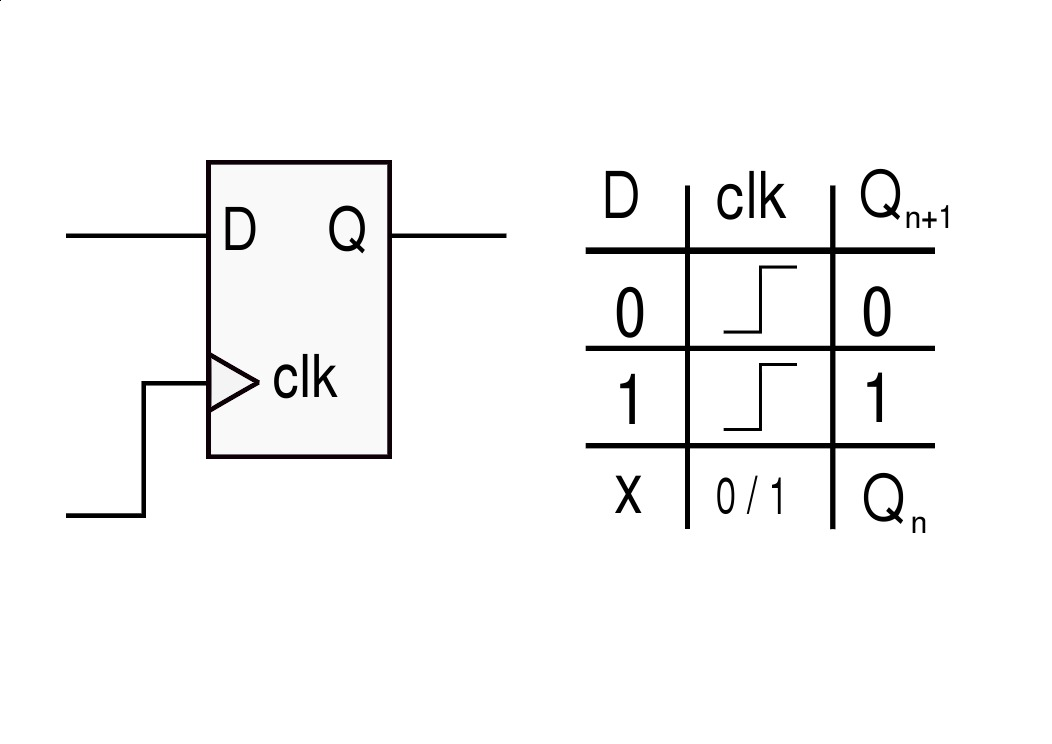
\includegraphics[scale=0.2]{./images/d-ff-infos.jpg}
\end{figure}

La bascule D a pour fonction de recopier l'entrée $D$ sur sa sortie $Q$, lors d'un court temps d'échantillonnage : il s'agit généralement du \textbf{front montant} de l'horloge. Cette horloge est supposée périodique. Pour que l'échantillonnage se passe correctement \textit{d'un point de vue physique}, le signal d'entrée doit respecter deux contraintes : il doit être parfaitement stable \textit{un peu avant} et \textit{un peu après} le front montant. Ces instants s'appellent temps de \textit{setup} et temps de \textit{hold}. La donnée est électriquement recopiée après un instant également très court appelé ``clock to Q''. Tous ces temps sont très inférieurs à la période d'horloge.\\

\textbf{La bascule D permet ainsi de travailler sur un signal stable, pendant toute une période} : le temps est désormais \textbf{discrétisé}. Il n'y a plus à se soucier des temps de propagation caractéristiques -- et parfois fluctuants -- des différentes portes logiques réalisant les calculs ! Il suffit d'attendre une période d'horloge suffisamment longue pour observer un résultat combinatoire correct, échantillonné dans une bascule. L'horloge absorbe ces variations : c'est l'\textit{hypothèse synchrone}. L'écoulement du temps ne se fait que par ``quantum'' de temps : celui des ``tops'' (ou ``ticks'') de cette horloge périodique.\\

Il est même possible d'abstraire le fonctionnement du circuit encore plus en supposant que seuls ces instants d'échantillonnage sont significatifs et que les calculs s'effectuent instantanément sur ces ``tops'' (on parle de calcul en ``temps zéro''), et que rien ne se passe entre ces ``tops'' ! Mais cela reste ``une vue de l'esprit'' : c'est un des nombreux mécanismes d'\textit{abstraction} rencontrés en conception de circuits numériques.

\vspace{1em}
\noindent\textbf{Exercice :} Compléter le chronogramme suivant où un signal $S_1$ sur 4 bits, extérieur au système et asynchrone, est fourni comme entrée (sous sa forme entière).

\begin{figure}[H]
\centering
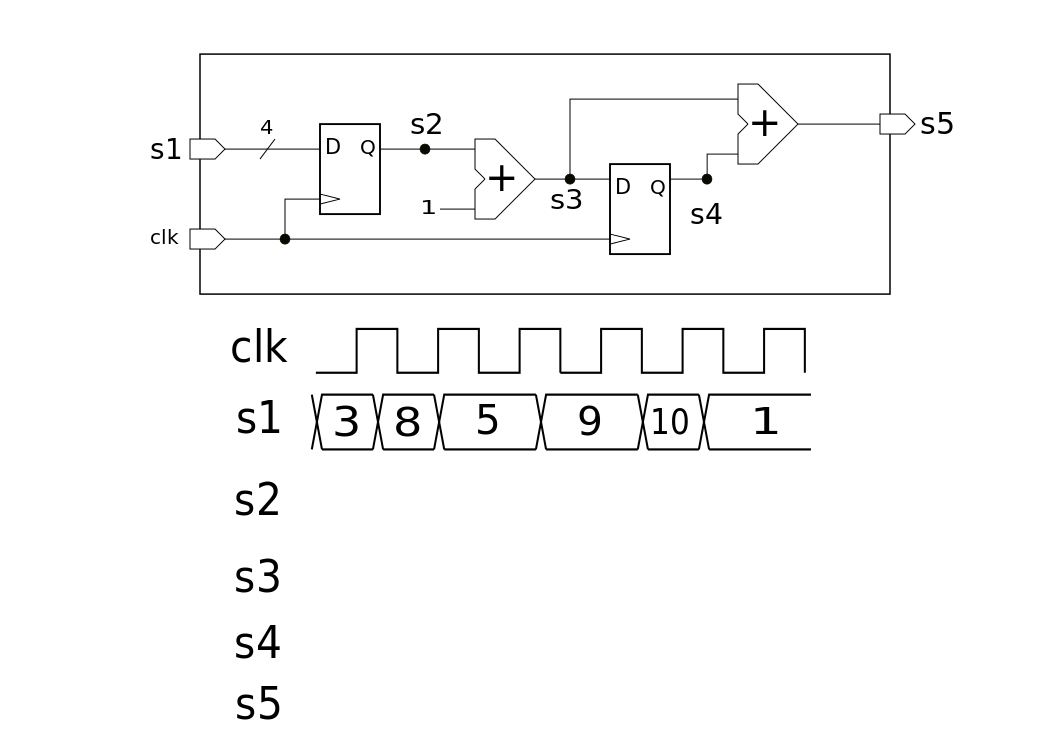
\includegraphics[scale=0.4]{./images/dff-1.png}
\end{figure}

On précise ici que :
\begin{itemize}
    \item nous ne tenons pas compte de la notion de temps de \textit{setup} et temps de \textit{hold}, ni du temps $t_{clk \to Q}$ ;
    \item les zones de transition des 4 bits se présentent ici comme des ``X'' ;
    \item pour les signaux internes au système, on ne représentera pas ces transitions, supposées idéales : seuls des rectangles suffiront ;
    \item on suppose que les sorties $Q$ sont initialisées à 0.
\end{itemize}

\ifsolutions
\begin{solbox}
\centering
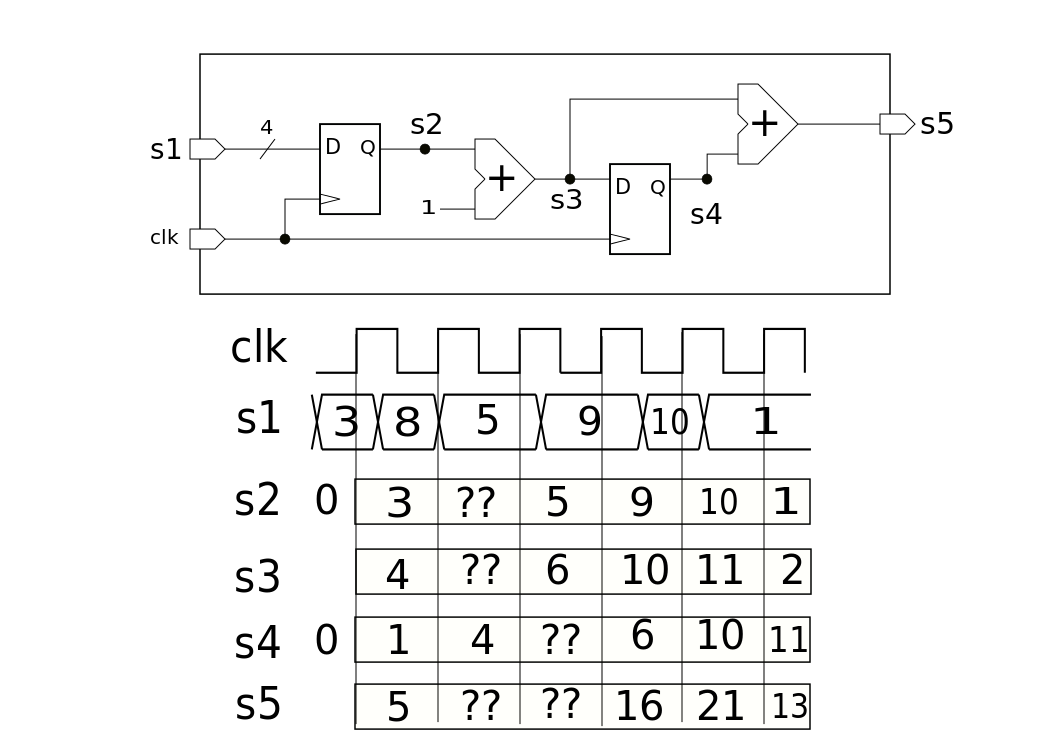
\includegraphics[scale=0.4]{./images/dff-1-CORR-1.png}
\captionof{figure}{Chronogramme complété}

\vspace{1em}
Les plus observateurs noteront que le signal $S_5$ possède deux valeurs $16$ et $21$ qui ne peuvent pas être encodées sur 4 bits (il en faut 5). Toutefois, dans cet exercice, rien ne stipule que tous les signaux doivent forcément être encodés sur 4 bits. Malgré tout, si on impose cette contrainte de 4 bits sur tous les signaux, ces deux valeurs seront tronquées : $16$ sera tronqué à $0$ et $21$ sera tronqué à $5$. Dans les deux cas, le MSB à 1 en position 5 est perdu.

\vspace{0.5em}
Une autre question récurrente sur cet exercice est la suivante : on a expliqué que l'échantillonnage de $S_1$ ne peut pas bien se passer sur la valeur incertaine entre 8 et 5. Le déclenchement de la recopie, par la bascule, sur front montant intervient sur un signal instable et dont la valeur ne peut être connue avec certitude. Pourtant, la solution proposée à l'exercice conduit à dessiner de tels cas, partout dans le tableau : les transitions entre les valeurs sont inscrites sur le front lui-même, ce qui a de quoi perturber\ldots

\vspace{0.5em}
En réalité, la bascule D possède deux fonctions :
\begin{itemize}
    \item vis-à-vis d'un signal externe (comme $S_1$), non synchronisé sur l'horloge, la bascule permettra de filtrer le signal, en ne conservant que les valeurs se prêtant à un échantillonnage correct (respect des temps de setup et de hold) ;
    \item ensuite, en interne, la bascule D réalise la simple recopie de l'entrée, décalée d'un cycle d'horloge.
\end{itemize}
\end{solbox}

\begin{solbox}
Une autre manière de voir les choses, et qui permet d'éviter de considérer deux fonctions distinctes à la bascule, est d'insérer des temps $\delta t_i$ infinitésimaux entre l'instant précis du front montant et l'apparition de la valeur sur $Q_i$. Physiquement, ces temps existent (clk-to-Q). Toutefois, il est préférable de ne plus les considérer (on les fait tendre vers 0) : cela permet de simplifier les raisonnements, en retombant dans le monde des suites numériques, plutôt que de conserver ces grandeurs temporelles physiques, par ailleurs compliquées à dessiner !

Il s'agit d'une abstraction, qui fonctionne très bien dans le cas des circuits numériques synchrones. Pour rappel, une abstraction cherche à gommer les détails inutiles (ici le temps physique), tout en conservant les propriétés essentielles (ici la recopie) de l'objet considéré (la bascule).
\end{solbox}
\fi

%\newpage

\section{Du circuit au chronogramme}

Soit le circuit logique suivant.

\begin{figure}[H]
\centering
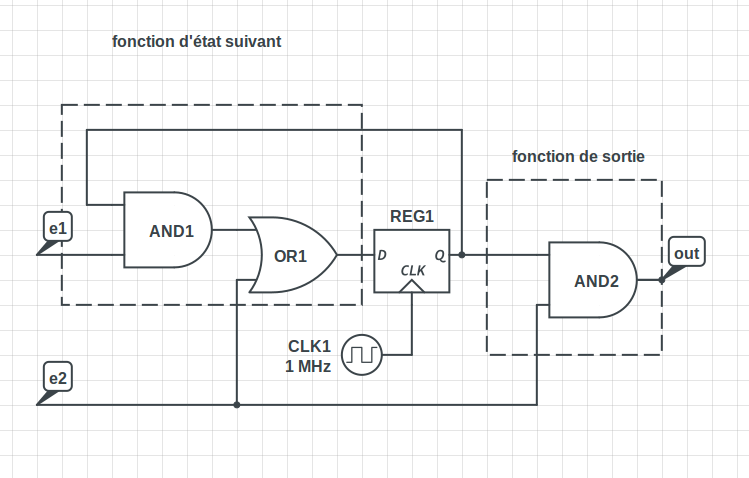
\includegraphics[scale=0.3]{./images/fsm-ex1.png}
\end{figure}

Sachant que la bascule D est initialisée à 0, trouver le chronogramme de la sortie $out$ correspondante, lorsque les valeurs d'entrée sont (respectivement, à chaque coup d'horloge) :

\begin{lstlisting}
e1 : 0 1 0 1 1 0 1
e2 : 1 1 1 0 1 0 0
\end{lstlisting}

\ifsolutions
\begin{solbox}
On commence par le cycle 1 : on connaît la valeur de $e_1=0$ à ce cycle, ainsi que la valeur $Q=0$ (comme indiqué dans l'énoncé). On en déduit : la sortie du ET vaut $0$. D'où, connaissant $e_2=1$, on trouve la sortie du OU égale à $1$. Cette sortie du OU est également l'entrée $D$ de la bascule. Enfin, pour ce premier cycle, on détermine la sortie OUT, qui vaut $0$.

On peut donc passer au cycle 2 : pour cela il faut commencer par dépercuter la valeur précédente ($1$) sur $D$ vers la sortie $Q$ courante de la bascule. Ainsi, $Q$, au cycle 2, vaut $1$. À partir de là, on peut continuer à propager les calculs, de proche en proche.

Un calcul combinatoire impose de rester dans l'instant courant, alors qu'un élément séquentiel (bascule D) impose de se déplacer dans le temps, discrétisé.

On trouve le chronogramme complet :

\vspace{0.5em}
\begin{center}
\renewcommand{\arraystretch}{1.2}
\begin{tabular}{c c c c c c c c}
\toprule
\textbf{Cycle} & 1 & 2 & 3 & 4 & 5 & 6 & 7 \\
\midrule
$e_1$ & 0 & 1 & 0 & 1 & 1 & 0 & 1 \\
$e_2$ & 1 & 1 & 1 & 0 & 1 & 0 & 0 \\
\textsc{and} & 0 & 1 & 0 & 1 & 1 & 0 & 0 \\
\textsc{or}  & 1 & 1 & 1 & 1 & 1 & 0 & 0 \\
$D$ & 1 & 1 & 1 & 1 & 1 & 0 & 0 \\
$Q$ & 0 & 1 & 1 & 1 & 1 & 1 & 0 \\
\textsc{out} & 0 & 1 & 1 & 0 & 1 & 0 & 0 \\
\bottomrule
\end{tabular}
\end{center}
\end{solbox}
\fi

%\newpage

\section{Du chronogramme au circuit}

Nous proposons ici un exercice plus rare, uniquement par jeu : il s'agit de retrouver le circuit qui a généré les chronogrammes suivants. Il y a probablement plusieurs solutions ! Soyez perspicaces ! Les signaux $e_i$ représentent des entrées, les signaux $s_i$ des sorties, et les signaux $n_i$ des signaux internes.

\begin{lstlisting}
e1 : 0 0 1 1 0 0 0 0 1 1 0 0 1 0 0 0 0
e2 : 0 0 0 0 1 0 0 1 0 1 1 0 1 1 0 0 0
n1 : 0 0 1 1 1 0 0 1 1 1 1 0 1 1 0 0 0
s1 : 0 0 1 0 0 0 0 1 0 0 0 0 1 0 0 0 0
s2 : 1 1 0 1 1 1 1 0 1 1 1 1 0 1 1 1 1
s3 : ? 1 1 0 1 1 1 1 0 1 1 1 1 0 1 1 1
\end{lstlisting}

\ifsolutions
\begin{solbox}
On voit que :
\begin{itemize}
    \item $n_1$ est le OU entre $e_1$ et $e_2$ ;
    \item $s_1$ marque le début de la séquence des 1 de $n_1$ : $s_1 = n_{1,t} \cdot \overline{n_{1,t-1}}$ (front montant) ;
    \item $s_{2,t}$ est l'inverse de $s_{1,t}$ ;
    \item $s_3$ est égal au signal $s_2$, décalé d'un cycle : $s_{3,t} = s_{2,t-1}$.
\end{itemize}

Un circuit possible est alors :

\vspace{0.5em}
\centering
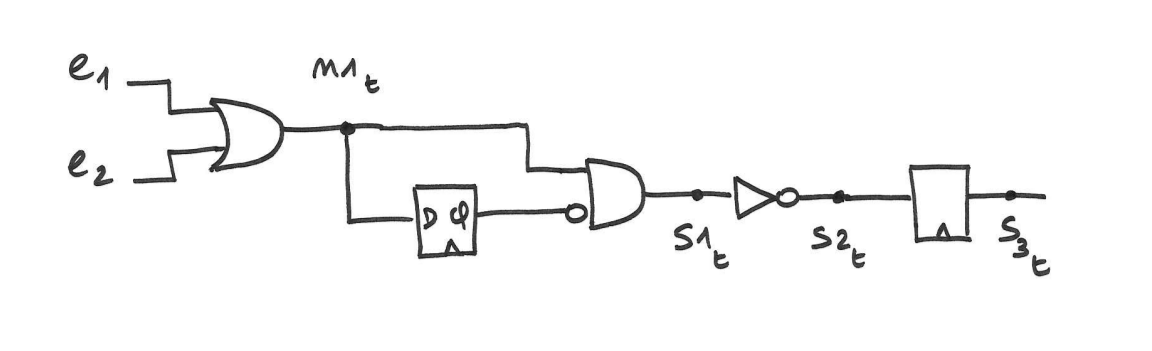
\includegraphics[scale=0.3]{./images/exo5-circuit.png}
\captionof{figure}{Circuit proposé pour reproduire les chronogrammes}
\end{solbox}
\fi

% Section commentée dans l'original, conservée telle quelle
% \section{Du circuit au diagramme à bulles}
% ...

%\newpage

\section{Suite de Fibonacci en circuit}

La suite de Fibonacci est bien connue : $u_{n+2}=u_{n+1}+u_{n}$, où $u_{1}=1$ et $u_0=0$. Elle date de 1202 et décrit la croissance d'une population de lapins, à partir d'un seul couple. Pour la petite histoire, cette suite a par ailleurs un lien étonnant avec le nombre d'or $\phi=\frac{1+\sqrt{5}}{2} \approx 1{,}618$. En effet, Euler a démontré que pour un $n$ donné (un ``step''), on a :
$$u_n=\frac{1}{\sqrt{5}}\left(\phi^n - \phi'^n\right) \quad \text{où} \quad \phi' = -\frac{1}{\phi}$$

\begin{enumerate}
    \item Dessiner le circuit numérique émettant la suite de Fibonacci. Un changement d'indice simple, au préalable, est conseillé.
    \item Chaque bascule D possède un reset actif haut, et un set actif bas. Compléter le schéma précédent, de manière à initialiser correctement les bascules. On dispose d'un bouton poussoir d'initialisation qui fournit un signal de \textit{reset} actif \textit{haut} : lorsqu'on appuie sur ce bouton pour initialiser le circuit, ce signal vaut ``1''.
\end{enumerate}

\ifsolutions
\begin{solbox}
\begin{enumerate}
    \item On fait le changement d'indice suggéré : $u_n=u_{n-1}+u_{n-2}$. Le décalage temporel correspond à une bascule D. On a donc le schéma ci-dessous. On a omis le signal d'horloge, supposé présent de manière implicite.

    \vspace{0.5em}
    \centering
    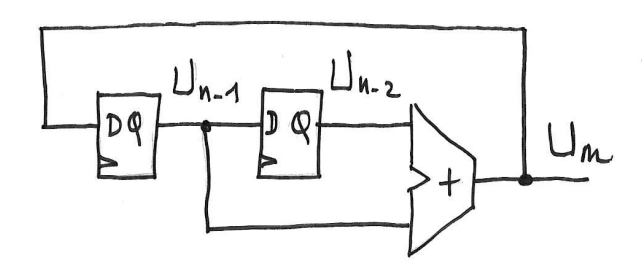
\includegraphics[scale=0.3]{./images/fibo1.png}
    \captionof{figure}{Circuit générateur de la suite de Fibonacci}
    \label{fibo1}

    \item L'initialisation se fait comme présenté sur le schéma ci-dessous.

    \vspace{0.5em}
    \centering
    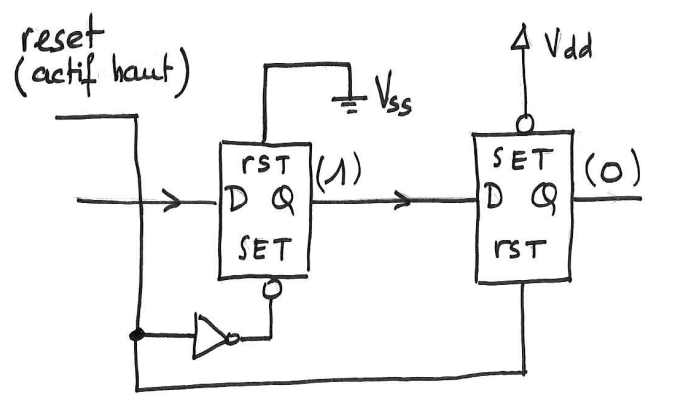
\includegraphics[scale=0.3]{./images/fibo2.png}
    \captionof{figure}{Circuit avec initialisation par reset/set}
    \label{fibo2}
\end{enumerate}
\end{solbox}
\fi



\part{Chemin de données ou \textit{datapath}}

Nous avons déjà abordé la notion de ``chemin de données'' dans le ``jeu des cambrioleurs'' (TD1) : il s'agissait uniquement d'acheminer, en combinatoire, une donnée d'une entrée vers une sortie, sans traitement spécifique. En général, les \textit{datapaths} sont plus complexes et associent à la fois logique séquentielle et logique combinatoire. Ils constituent le coeur des architectures de calculs.

L'essentiel de leur puissance de calcul provient de deux notions fondamentales :
\begin{itemize}
    \item \textbf{Le parallélisme} : il s'agit d'effectuer plusieurs opérations durant un seul cycle d'horloge, grâce à l'utilisation de plusieurs opérateurs matériels. Pour rappel, dans un processeur classique (et comme dans les langages dits ``séquentiels''), les opérations se font en séquence, les unes à la suite des autres. Ici, à l'inverse, nous sommes en mesure de construire des calculateurs qui effectuent plusieurs opérations simultanément.
    \item \textbf{Le pipeline} : il s'agit d'effectuer des opérations ``à la chaîne'', sur des données, chaque \textit{étage} du pipeline ayant une action spécifique sur ces données.
\end{itemize}

Nous allons d'abord chercher à illustrer le rôle de la bascule D dans la structure d'un pipeline élémentaire : le registre à décalage.

\section{Pipeline, Registres à décalage et Applications}

Le registre à décalage le plus simple consiste à relier la sortie d'une première bascule D à l'entrée d'une seconde bascule D. Ceci se généralise à un nombre $L$ de bascules ainsi enchaînées les unes aux autres (sans rebouclage). Une donnée $e$ qui se présente au cycle $n$ mettra $L$ cycles (ou ``coups d'horloge'') à parvenir à la sortie $s$.

Sa fonction est double :
\begin{enumerate}
    \item Retarder la donnée $a_0$ d'un temps discret $L$ : elle se présente sur l'entrée $e$ au temps $t$ et ressort sur la sortie $s$ du dispositif au temps $t+L$.
    \item Autoriser une donnée $a_1$ à se présenter sur l'entrée $e$ au temps $t+1$, en même temps que $a_0$ est échantillonnée par la seconde bascule, etc.
\end{enumerate}

\subsection*{Exercice 1 : registre à décalage simple}
Dessiner un registre à décalage de taille 4. Nommer correctement ses signaux et écrire l'équation de la sortie $s(t)$.

\ifsolutions
\begin{solbox}
\centering
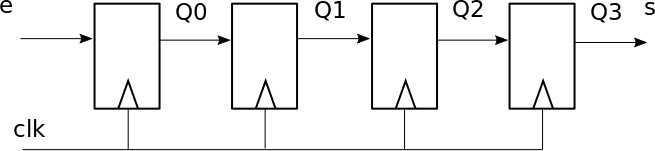
\includegraphics[scale=0.4]{./images/reg_dec.png}
\captionof{figure}{Registre à décalage de profondeur 4.}
\label{rec_dec}

\vspace{0.5em}
L'équation de sortie est :
$$ s(t) = e(t-4) $$

Le chronogramme est le suivant :
\begin{center}
\renewcommand{\arraystretch}{1.2}
\begin{tabular}{c c c c c c c c}
\toprule
\textbf{Cycle} & 0 & 1 & 2 & 3 & 4 & 5 & \dots \\
\midrule
$e$ & $a_0$ & $a_1$ & $a_2$ & $a_3$ & $a_4$ & $a_5$ & \dots \\
$s$ & ? & ? & ? & ? & $a_0$ & $a_1$ & \dots \\
\bottomrule
\end{tabular}
\end{center}
\end{solbox}
\fi

\subsection*{Exercice 2 : registre à décalage commandé}
Modifier le registre à décalage précédent de manière à le commander par un signal \texttt{push}, qui autorise les données à s'acheminer progressivement vers la sortie lorsque ce signal vaut ``1''.

\ifsolutions
\begin{solbox}
\centering
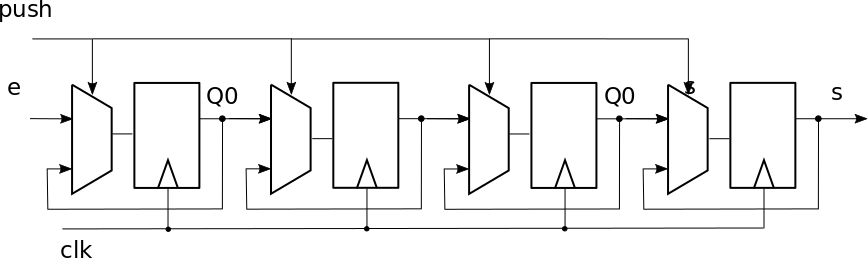
\includegraphics[scale=0.4]{./images/reg_dec_ctrl.png}
\captionof{figure}{Registre à décalage de profondeur 4, avec signal de contrôle \texttt{push}.}
\label{rec_dec_ctrl}
\end{solbox}
\fi

\subsection*{Exercice 3 : moyenne mobile}
Soit un flux séquentiel de données (boursier, médical, etc.), dont les données successives arrivent au rythme de 100 MHz. La moyenne mobile (ou moyenne glissante, ou \textit{sliding average} en anglais) d'un tel flux continu permet de lisser une moyenne au cours du temps.

\begin{enumerate}
    \item Calculer rapidement la moyenne mobile, sur 4 échantillons, du flux suivant : $$\dots, 0, 0, 0, 0, 8, 9, 13, 4, 3, 2, 1, 0, 0, 0, \dots$$
    \item Concevoir un circuit numérique qui réalise le calcul d'une moyenne mobile sur 4 échantillons de nombres entiers, supposés non signés. Proposer une seconde solution. Laquelle est meilleure ? On s'autorise à utiliser la notion d'additionneur, mais pas de diviseur.
    \item Combien de bits sont nécessaires pour calculer la somme de 4 données codées sur 8 bits ? Combien pour la moyenne mobile ?
    \item Combien de bits sont nécessaires pour calculer la somme de $n$ données codées sur $m$ bits ?
    \item Sachant que le temps de traversée de l'additionneur est 4 ns, quelle est la fréquence atteignable du circuit ? Est-ce compatible avec la fréquence d'arrivée des données ?
\end{enumerate}

\ifsolutions
\begin{solbox}
\begin{enumerate}
    \item La moyenne donne : $$\dots, ?, ?, ?, 0, 2, 4, 7, 8, 7, 5, 2, 2, 0, 0, \dots$$

    \item Une solution consiste à réaliser les additions en parallèle. Une seconde à les chaîner. Il n'y a pas de meilleure solution, tant que la fréquence du circuit est atteinte. Il faut pour cela calculer le chemin critique dans les deux cas.

    \item On se convainc assez facilement que pour 4 données de 8 bits, il faut \textbf{10 bits}. Pour la moyenne mobile on est ramené à \textbf{8 bits}.

    \item Soit $D(x)$ le nombre de bits nécessaire pour coder $x$ (entier positif non signé). On a $D(x) = \lfloor \log_2(x) + 1 \rfloor$. Pour l'addition $S$ de $n$ données codées sur $m$ bits, on a donc :
    $$ D(S) = \lfloor \log_2(n \cdot (2^m - 1)) + 1 \rfloor $$

    \item $4 + 4 = 8$ ns. On inverse : la fréquence atteignable est de $\mathbf{125\ MHz}$ au maximum. C'est parfaitement compatible avec la fréquence de 100 MHz : il faudra veiller à ce que le circuit fonctionne exactement à la même fréquence que l'émetteur des données.
\end{enumerate}
\end{solbox}
\fi

\subsection*{Exercice 4 : look-up table de FPGA}
Les FPGA sont des circuits réguliers qui ont l'étonnante propriété d'être reprogrammables à volonté. On parle de ``circuits reconfigurables''. Les FPGA sont constitués d'un assemblage de briques élémentaires appelées BLE (\textit{Basic Logic Element}), interconnectées en réseau. Leur topologie détaillée est présentée dans le polycopié du cours.

Un BLE se compose notamment d'une LUT (\textit{look-up table}) à $n$ entrées : c'est une mémoire qui permet d'enregistrer les valeurs attendues de n'\textit{importe quelle fonction booléenne à $n$ entrées}. C'est l'équivalent matériel d'une petite table de vérité, qui se présente sous la forme d'un registre à décalage \textit{avec \texttt{enable}} (voir exercice précédent où on a appelé ce signal \texttt{push})\footnote{\dots pour les besoins de notre exercice. Les LUTs des FPGAs sont réalisées au niveau transistors.} à $2^n$ bascules : le flux qui entre dans ce registre à décalage s'appelle un \textit{bitstream}. Il agit comme une programmation ou \textit{configuration} de la LUT.

Chaque sortie $Q_i$ des bascules de la LUT est connectée à une des $2^n$ entrées d'un multiplexeur. Les signaux de contrôle du multiplexeur sont les $n$ entrées, notées ici $\{a, b, c, \dots, \alpha_{n-1}\}$.

\begin{enumerate}
    \item Dessiner une LUT 2.
    \item On suppose que le bitstream est entré à l'aide d'un signal de contrôle auxiliaire \texttt{push} (cf exercice 2) de la manière suivante : $1000$, où le bit le plus à droite représente la première donnée. Calculer la sortie du multiplexeur pour les combinaisons des entrées $a, b$.
    \item Quelle est la fonction réalisée par le dispositif ?
    \item Conclure en proposant un bitstream pour la fonction $xor(a,b)$.
\end{enumerate}

\ifsolutions
\begin{solbox}
\begin{enumerate}
    \item Voir figure \ref{lut}.

    \vspace{0.5em}
    \centering
    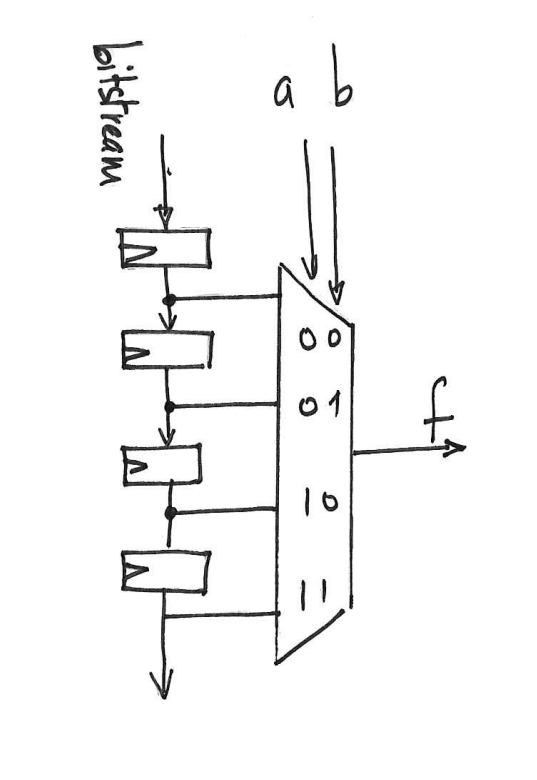
\includegraphics[scale=0.2]{./images/lut.png}
    \captionof{figure}{LUT2 (2 entrées) -- On a omis le bit \texttt{enable} (ou \texttt{push}) pour simplifier le schéma, mais ce contrôle est nécessaire afin de bien séparer les phases de programmation (\textit{configuration}) et d'utilisation.}
    \label{lut}

    \item Les combinaisons de sortie sont :
    \begin{center}
      \renewcommand{\arraystretch}{1.2}
      \begin{tabular}{c c c}
        \toprule
        $a$ & $b$ & $f$ \\
        \midrule
        0 & 0 & 1 \\
        0 & 1 & 0 \\
        1 & 0 & 0 \\
        1 & 1 & 0 \\
        \bottomrule
      \end{tabular}
    \end{center}

    \item C'est la fonction \textbf{NOR2}. Le bitstream nous a permis de configurer la LUT en NOR2 !

    \item Pour un XOR, le bitstream est $\mathbf{0110}$.
\end{enumerate}
\end{solbox}
\fi
\end{document}
